\chapter{Ocena aplikacji}
\label{cha:ocena}

W tym rozdziale zaprezentowana została kompleksowa ocena aplikacji \en. Jest ona
podzielona na kilka części. Następnie zaprezentowane są testy jakościowe, które
opierają się na próbie odzwierciedlenia wybranych zjawisk fizycznych przy pomocy
symulatora. Z kolei testy wydajnościowe wersji podstawowej oraz równoległej \en
pokazują zysk jaki dało przeniesienie obliczeń na kartę graficzną. Na podstawie
tych wyników zanalizowana została dostępność aplikacji dla potencjalnych
użytkowników na różnych urządzeniach oraz ich konfiguracjach. Rozdział kończy
ocena stopnia realizacji założeń projektowych oraz krótkie podsumowanie.

\section{Modelowanie wybranych zjawisk fizycznych jako testy jakościowe symulatora}

W przypadku aplikacji edukacyjnej jaką jest symulator \en niezwykle istotne jest
aby symulowane zjawiska odzwierciedlały w sposób  wiarygodny rzeczywistość. Z
drugiej jednak strony, aplikacja musi być interaktywna i działać w czasie
rzeczywistym. Dlatego też nie można sobie pozwolić na zbyt długi czas
wykonywania, co zwykle idzie w parze z dokładnymi algorytmami i obliczeniami. Z
tego też powodu zastosowane silniki (algorytmy) fizyczne balansują pomiędzy
poprawnością fizyczną, a wydajnością (por. rozdział \ref{sec:silnikiFizyczne}).
Jest to dopuszczalne, ponieważ symulacja jest zorientowana wyłącznie na aspekt
wizualny.

Z powodu tego kompromisowego podejścia do pełnej dokładności obliczeń, niezwykle
istotne były testy aplikacji pod kątem podstawowej poprawności fizycznej. W tym
celu zostały przygotowane przypadki testowe, które miały za zadanie modelować
powszechnie znane zjawiska fizyczne związane z przewodnictwem cieplnym oraz
dynamiką płynów. Poniżej przedstawione są wyniki tych testów.

\subsection{Komórki Bénarda}

Modelowanie komórek Bénarda to jeden z podstawowych testów aplikacji
symulujących dynamikę płynów. Są to komórki konwekcyjne powstające w płynie
podgrzewanym od spodu. Rysunek \ref{fig:physBenard} prezentuje wyniki symulacji
przeprowadzonej przez \en.

\begin{figure}[!h]
\centering
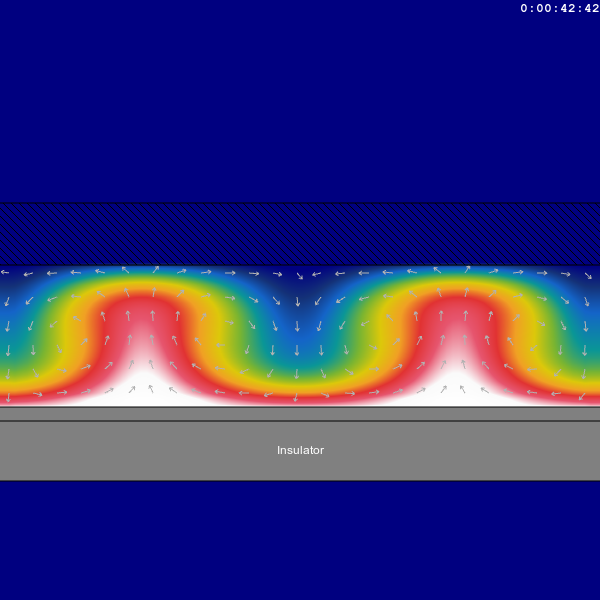
\includegraphics[width=0.8\textwidth]{img/physics/benard}
\caption{Symulacja formowania się komórek Bénarda}
\label{fig:physBenard}
\end{figure}

Wyraźnie widać formowanie się oczekiwanych komórek. Ich układ oraz kształt
stabilizuje się po bardzo krótkim czasie symulacji. Wyniki można uznać za w
pełni satysfakcjonujące.

\subsection{Przepływ laminarny oraz turbulentny}
\label{sec:przeplywyLamTur}

Symulacja przepływów laminarnych oraz turbulentnych to następny test silnika
dynamiki płynów. Rodzaj przepływu, w przypadku gdy jest on zakłócony przez
obecność przeszkody, w głównym stopniu determinuje liczba Reynoldsa. Jest ona
zależna od:

\begin{itemize}
\item lepkości płynu,
\item prędkości przepływu,
\item średnicy przeszkody.
\end{itemize}

W związku z tym został przygotowany przypadek testowy, w którym płyn ma stałą
lepkość, a przeszkody identyczne wymiary. Zmienna jest tylko prędkość przepływu.
Dla mniejszych prędkości oczekiwanym wynikiem był przepływ laminarny, dla
większych przepływ turbulentny. Rysunek \ref{fig:physLaminarTurbulent}
prezentuje wyniki takiej symulacji przeprowadzonej przez \en.

\begin{figure}[!h]
\centering
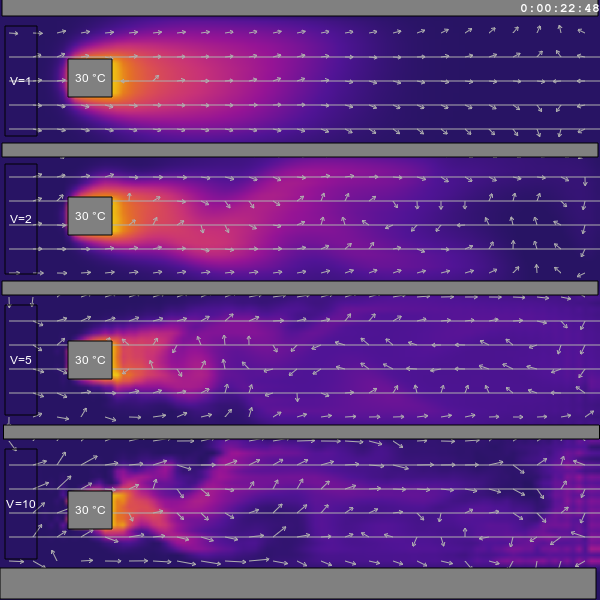
\includegraphics[width=0.8\textwidth]{img/physics/laminarTurbulent}
\caption{Symulacja wpływu liczby Reynoldsa na rodzaj przepływu}
\label{fig:physLaminarTurbulent}
\end{figure}

Rezultaty są zgodne z oczekiwaniami. Wyraźnie widać wpływ liczby Reynoldsa
(determinowanej przez prędkość płynu) na rodzaj przepływu.

\subsection{Ścieżka wirowa von Kármána}

Ścieżka wirowa von Kármána to kolejny doskonały test silnika dynamiki płynów.
Jest to szczególny rodzaj przepływu turbulentnego, który powstaje wyłącznie dla
pewnego zakresu wartości liczby Reyonldsa (por. \ref{sec:przeplywyLamTur}).

W związku z tym został przygotowany przypadek testowy, w którym płyn ma stałą
lepkość oraz prędkość przepływu, natomiast zmienna jest tylko średnica
przeszkody. Zgodnie z powyższymi założeniami, powinno być możliwe dobranie
takich średnic przeszkód, aby wiry Kármána powstały tylko za większą z nich.
Rysunek \ref{fig:physKarman} prezentuje wyniki takiej symulacji przeprowadzonej
przez \en.

\begin{figure}[!h]
\centering
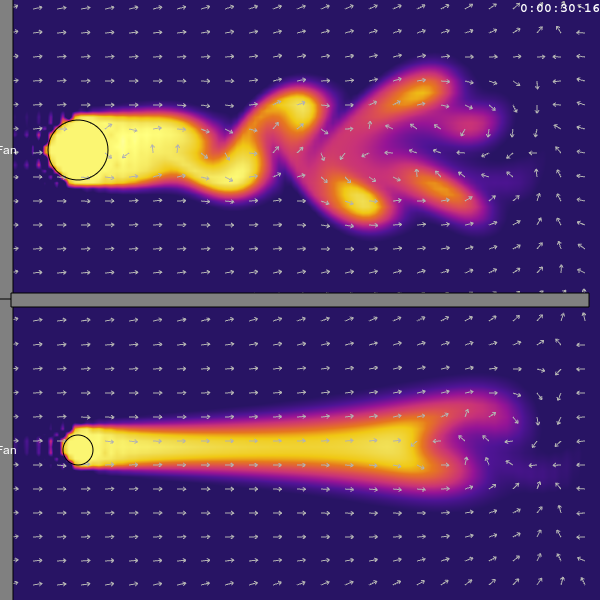
\includegraphics[width=0.8\textwidth]{img/physics/karman}
\caption{Symulacja formowania się wirów Kármána}
\label{fig:physKarman}
\end{figure}

Rezultaty są zgodne z oczekiwaniami. Wir powstał tylko w warunkach, w których
liczba Reynoldsa była większa.

\subsection{Pojemność cieplna}

Tym razem przypadek testowy dotyczy silnika przewodnictwa cieplnego. Pojemność
cieplna jest wielkość fizyczna, która charakteryzuje ilość ciepła, jaka jest
niezbędna do zmiany temperatury ciała o jednostkę temperatury. Poprawna
symulacja powinna uwzględniać ten parametr materiałów.

Aby to sprawdzić przygotowany został przypadek testowy, w którym znajdują się
dwa materiały o różnej pojemności cieplnej. Materiał o większej pojemności
powinien przewodzić ciepło znacznie lepiej niż ten o pojemności mniejszej.
Wyniki takiego eksperymentu przeprowadzonego przez symulator \en prezentuje
rysunek \ref{fig:heatCapacity}.

\begin{figure}[!h]
\centering
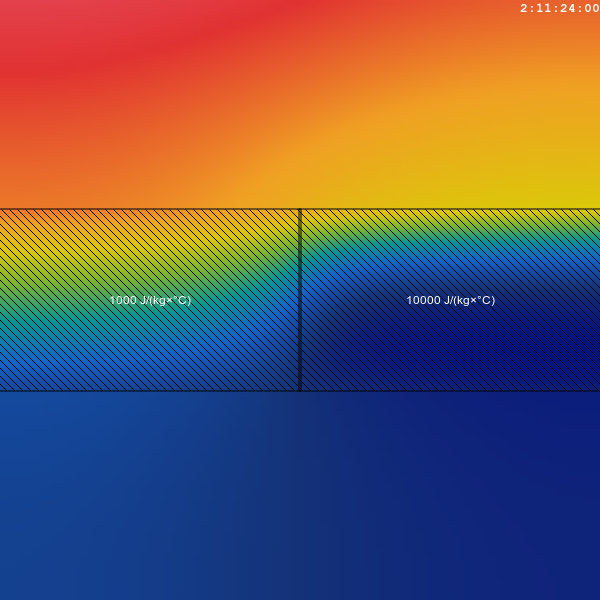
\includegraphics[width=0.8\textwidth]{img/physics/heatCapacity}
\caption{Symulacja wpływu pojemności cieplnej na przewodnictwo cieplne}
\label{fig:heatCapacity}
\end{figure}

Rezultaty po raz kolejny są zgodne z oczekiwaniami. Widać wyraźnie, iż materiał
o większej pojemności cieplnej znacznie lepiej przewodzi ciepło.

\subsection{Aspekt edukacyjny}

Ostatni z zaprezentowanych testów jest bardziej złożony. Nie prezentuje on
jednego, konkretnego zjawiska fizycznego jak poprzednie przykłady. Skupia się on
na zaprezentowaniu przykładowych możliwości symulacji oraz na potencjalnym
aspekcie edukacyjnym.

Przygotowana została scena zawierająca nieszczelnie izolowane pomieszczenie,
będące metaforą mieszkania. Jest ono ogrzewane przez element grzewczy o stałej
mocy. W jego otoczeniu został wymuszony dość mocny przepływ symulujący wiatr.
Miało to na celu pokazanie użytkownikom różnych, potencjalnych dróg ucieczki
ciepła z pomieszczeń mieszkalnych.

\begin{figure}[!h]
\centering
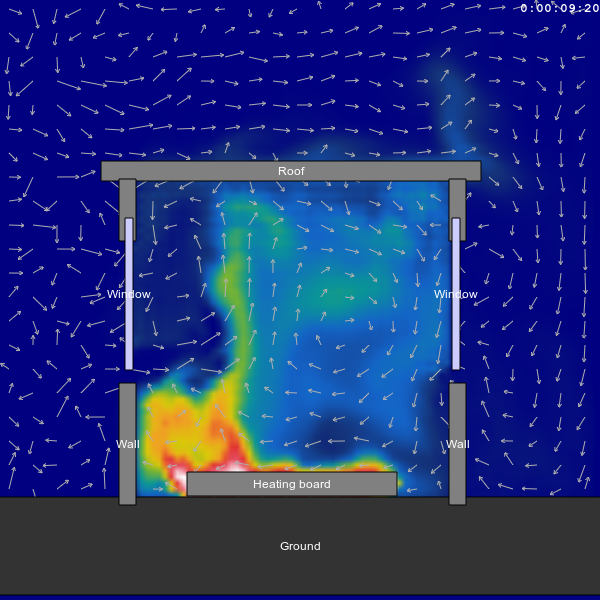
\includegraphics[width=0.8\textwidth]{img/physics/wind}
\caption{Symulacja ucieczki ciepła z pomieszczeń mieszkalnych}
\label{fig:wind}
\end{figure}

Rysunek \ref{fig:wind} prezentuje efekty takiej symulacji. Widoczne są dwa
wyraźne zjawiska -- strata ciepła w okolicy nieszczelnych okien oraz strata
ciepła związana z przewodnictwem cieplnym dachu. Pozwala to lepiej zrozumieć
użytkownikowi (docelowo uczniowi na początkowym etapie edukacji) wpływ różnych
aspektów pomieszczeń mieszkalnych (takich jak szczelność czy izolacja) na straty
ciepła. Może przyczynić się to do rozsądniejszego i ekonomiczniejszego
gospodarowania energią w jego własnym mieszkaniu czy też domu. W dobie
szczególnej dbałości o środowisko naturalne jest to niezwykle cenny i pożądany
efekt edukacyjny.

\section{Testy wydajnościowe}

Wydajność jest kluczowym aspektem symulacji ukierunkowanej na cele edukacyjne.
Tylko odpowiednia prędkość symulacji może przyciągnąć uwagę użytkownika i
zachęcić go do dalszej eksploracji zagadnienia.

W celu osiągnięcia zadowalającej wydajności na różnych urządzeniach zastosowano
kilka technik. Podstawową jest świadoma implementacja polegająca na unikaniu
zbędnych, czasochłonnych operacji, wynikająca ze znajomości środowiska
przeglądarki internetowej. Jednak krokiem, który najbardziej przyczynił się do
powstania naprawdę wydajnej aplikacji było przeniesienie obliczeń związanych
z fizyką na procesor karty graficznej.

Niniejsza sekcja przedstawia zyski z zastosowania tej optymalizacji. Omówiona
jest także kwestia wpływu konfiguracji sprzętowej użytkownika oraz związana z
tym ogólna dostępność symulatora dla szerokiego grona odbiorców.

\subsection{Konfiguracje sprzętowe przeznaczone do testów}

Testy zostały przeprowadzone na następujących komputerach:

\begin{enumerate}

\item Konfiguracja 1. -- 

\item Konfiguracja 2. -- 

\end{enumerate}

\subsection{Zysk wydajności wynikający z przeniesienia obliczeń na GPU}

\subsection{Wpływ optymalizacji i równoległości na jakość symulacji}

\section{Ocena dostępności aplikacji dla potencjalnych użytkowników}

\subsection{Wpływ posiadanej konfiguracji sprzętowej i oprogramowania na
symulator}

\section{Realizacja kluczowych wymagań}

\section{Podsumowanie}
